\chapter{Effective Field Theory}
\label{chap:EFT}

The concept of effective interactions has been around for nearly a century since Fermi first introduced it in 1933~\cite{Fermi:1933jpa} to explain the $\upbeta$ decay. Modern approach to effective interactions builds on the assumption that there is a separation between energy scales of different physics phenomena. When describing low-energy physics, the heavy mediators can be approximated to be point-like, and thus described by an effective coupling. This type of approaches, collectively known as \ac{EFT}, has been very successful in simplifying calculations and describing low-energy experiments with reasonably good precisions. Depending on the energy scale at which \acp{EFT} are operating, they can be classified in to different versions. One version of the \ac{EFT} that operates below the \ac{EW} scale and integrates out all the heavy fields is called the \ac{LEFT}, which is described in \autoref{sec:LEFT}. Another version of the \ac{EFT} that operators above the \ac{EW} scale is called the \ac{SMEFT}. It retains all the \ac{SM} fields and \sm~gauge symmetry. A description of the \ac{SMEFT} is given in \autoref{sec:SMEFT}.

\section{Low-Energy EFT}
\label{sec:LEFT}



\begin{figure}[tbh!]
 \begin{center}
 \begin{tabular}{cc}
 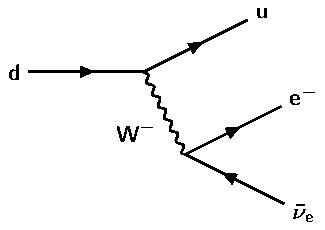
\includegraphics[width=0.45\textwidth]{figures/Part1/EFT/BetaDecay}&
 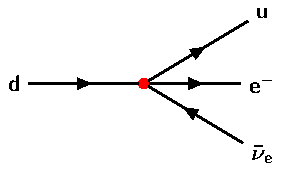
\includegraphics[width=0.45\textwidth]{figures/Part1/EFT/FermiTheory}\\
 \end{tabular}
 \caption{Representative Feynman diagrams for $\upbeta$ decay. The \ac{SM} description of this phenomenon with a massive weak mediator is illustrated on the left. At low energy, the heavy weak boson is approximated to be point-like in Fermi's theory of weak interactions, which is illustrated on the right. The effective coupling between four fermions, indicated with a red dot, can be used to describe the same phenomenon.}
 \label{fig:FermiEFT}
 \end{center}
\end{figure}

The \ac{LEFT} that we know today is not that different from Fermi's original theory of weak interactions. It makes no explicit assumptions about the structure of the theory at higher energy. Except for the gauge bosons, the Higgs boson, and the top quark fields, all other fields are considered in the \ac{LEFT}. 

The \ac{LEFT} is usually deployed in.a top down way to  

\begin{figure}[tbh!]
 \begin{center}
 \begin{tabular}{cc}
 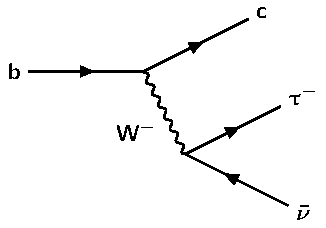
\includegraphics[width=0.45\textwidth]{figures/Part1/BSM/SMbtoc}&
 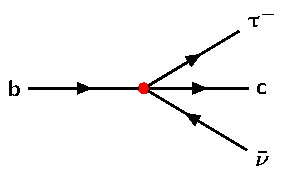
\includegraphics[width=0.5\textwidth]{figures/Part1/EFT/LEFT}
 \end{tabular}
 \caption{Representative Feynman diagram for $\rightarrow$c transtion in the \ac{SM} (left). This process might also be enhanced by new physics with a much higher energy scale. The potential contributions from new physics can therefore be described by an effective coupling between four fermions, which is illustrated on the right.}
 \label{fig:LEFT}
 \end{center}
\end{figure}

\section{Standard Model EFT}
\label{sec:SMEFT}

A different version of \ac{EFT}, known as \ac{SMEFT}, builds higher dimensional operators out of \ac{SM} fields. These higher dimensional operators respect \sm~gauge symmetry.